\section{Prototype}
\label{sec:prototype}

\subsection{Description}
\iLaTeX{} est un prototype d'éditeur de documents \LaTeX{} doté de représentations intermédiaires interactives.
Son interface ressemble à celle de la plupart des éditeurs \LaTeX{} traditionnels (code source à gauche, PDF généré à droite), mais certains éléments du PDF sont interactifs, de telle sorte qu'en cliquer un affiche la représentation intermédiaire associée au morceau de code qui l'a généré ({Figure~\ref{fig:ilatex-interface}}).
Cette visualisation peut alors être utilisée par les auteurs du document pour (1) visualiser des structures et des abstractions invisibles (\eg{} la grille d'un tableau sans bordure visible) et (2) modifier le code source du document (\eg{} réordonner les colonnes d'un tableau en manipulant sa grille).
Selon la position de l'élément cliqué sur l'écran, sa représentation intermédiaire est affichée au-dessus ou en-dessous de celui-ci, de façon à le laisser le plus visible possible.
Le reste du document est assombri jusqu'à ce que la représentation soit fermée en cliquant sur la croix ou sur le document assombri --- déclenchant alors une recompilation du document \LaTeX{} afin de mettre le PDF à jour.
En outre, chaque visualisation affiche le nom et la position du morceau de code visualisé dans son en-tête. Ceux-ci peuvent être cliqués afin d'afficher le code correspondant dans l'éditeur de code.
Nous avons implémenté trois types de RII : deux pour des éléments \LaTeX{} courants (images et tableaux), et une pour un élément personnalisé (une grille de mise en page).
Elles sont décrites plus en détail ci-après et illustrées par la {Figure~\ref{fig:ilatex-visualisations}}.

\begin{figure*}[h]
  \centering
  \iincludegraphics[width = \textwidth]{ilatex-interface.png}
  \caption{Interface du prototype. (1)~Éditeur de code; (2)~Pré-visualisation du PDF généré; (3)~Tableau disposant d'une RII (cliquable); (4)~Visualisation du code du tableau (affichée par dessus le PDF). La {Figure~\ref{fig:ilatex-visualisations}} illustre les différentes visualisations.}
  \label{fig:ilatex-interface}
\end{figure*}

\subsubsection{Détail des visualisations}

\paragraph{Images}
Les images sont détectées par l'utilisation de la commande \texttt{includegraphics} (telle que fournie par le paquet \texttt{graphicx}\footnote{\url{https://ctan.org/pkg/graphicx?lang=en}}).
La représentation intermédiaire d'une image ({Figure~\ref{subfig:ilatex-visualisation-image}}) affiche l'image à la même taille que l'image affichée dans le PDF.
Elle peut être redimensionnée (à l'aide de la molette de la souris) et rognée (en redimensionnant le masque représenté par le rectangle avec une bordure sombre et une poignée).
Ces manipulations mettent automatiquement à jour les paramètres de la commande en modifiant les valeurs des clés \texttt{width}, \texttt{height}, \texttt{trim} et \texttt{clip} (ou en les supprimant si elles ne sont plus nécessaires).
Cette visualisation répond principalement à la difficulté de visualiser et de formaliser des dimensions (\reftheme{4}), mais elle facilite également la découverte de certains paramètres utiles (\reftheme{2}).

\paragraph{Tableaux}
Les tableaux sont détectés par l'utilisation de l'environnement \texttt{tabular}.
Leur représentation intermédiaire ({Figure~\ref{subfig:ilatex-visualisation-tableau}}) affiche le contenu brut de chaque \og{} cellule \fg de l'environnement, qui peut être édité en double-cliquant sur la cellule.
Le type de chaque colonne est affiché dans une ligne d'en-tête, et les colonnes et les lignes peuvent être réordonnées en cliquant longuement sur leurs en-têtes respectives et en les déplaçant.
Cette visualisation permet de mettre en exergue une structure abstraite pouvant être invisible dans le PDF (\reftheme{4}).
Elle rend également des transformations telles que la réorganisation de colonnes beaucoup plus faciles qu'elles ne le seraient dans un éditeur de code (\reftheme{3}).

\paragraph{Grilles de mise en page}
Les grilles de mise en page sont détectées par l'utilisation de l'environnement \texttt{gridlayout}, un environnement personnalisé que nous avons développé afin d'illustrer l'utilité de \iLaTeX{} pour ce type de structure.
Il permet d'utiliser une grille de mise en page (constituée de lignes et de cellules), qui permet de disposer localement du contenu de type varié (\eg{} texte, images, tableaux) suivant une grille invisible.
La représentation intermédiaire ({Figure~\ref{subfig:ilatex-visualisation-grille}}) rend la grille visible.
Les cellules peuvent être redimensionnées horizontalement en faisant glisser leur bordure droite, et les lignes peuvent être redimensionnées verticalement en faisant glisser leur bordure inférieure.
En outre, cliquer une cellule affiche et sélectionne son contenu dans l'éditeur de code.
Cette visualisation supporte l'édition de contenu structuré (\reftheme{3}) et la représentation concrète d'abstractions telles que des dimensions relatives (\reftheme{4}).
Elle illustre également le potentiel de développement de nouvelles fonctionnalités pour \LaTeX{} dont l'utilisation serait plus difficile ou désagréable sans RII.


\begin{figure*}[h]
  \begin{gridlayout}{\textwidth}{10cm}
    \begin{row}{0.264}
      \begin{cell}{0.5}
        \raggedleft
        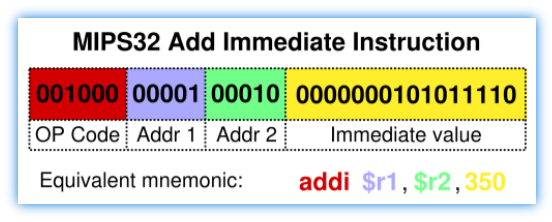
\includegraphics[height=\rowheight, width=\cellwidth, keepaspectratio]{image.png}
      \end{cell}
      \begin{cell}{0.5}
        \raggedright
        
\includegraphics[height=\rowheight, width=\cellwidth, keepaspectratio]{image-vis.png}
      \end{cell}
    \end{row}
    \begin{row}{0.268}
      \begin{cell}{0.5}
        \raggedleft
        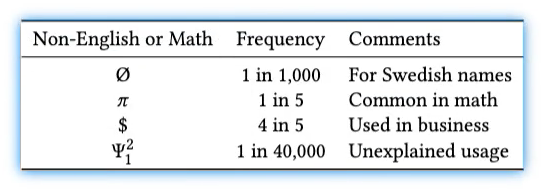
\includegraphics[height=\rowheight, width=\cellwidth, keepaspectratio]{table.png}
      \end{cell}
      \begin{cell}{0.5}
        \raggedright
        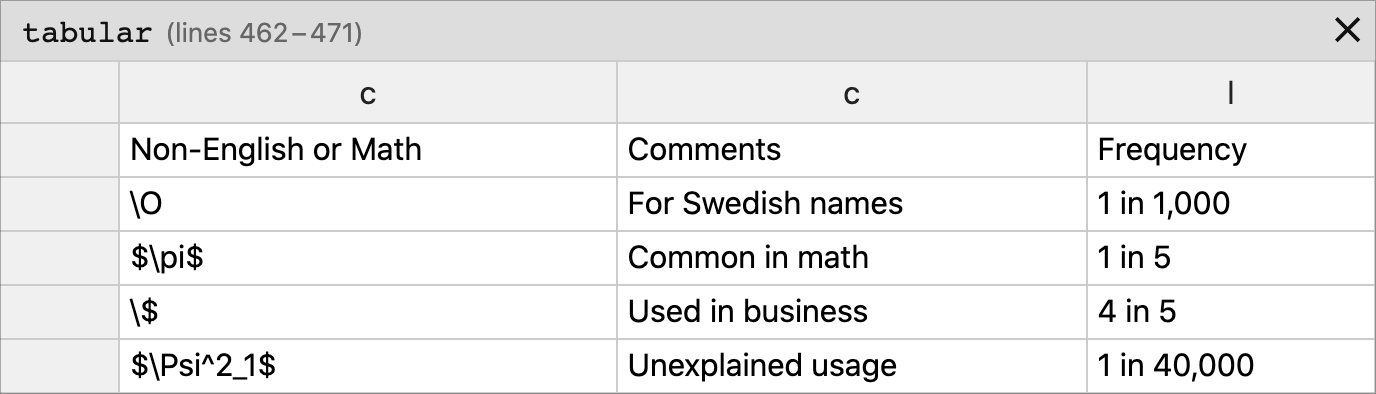
\includegraphics[height=\rowheight, width=\cellwidth, keepaspectratio]{table-vis.png}
      \end{cell}
    \end{row}
    \begin{row}{0.468}
      \begin{cell}{0.5}
        \raggedleft
        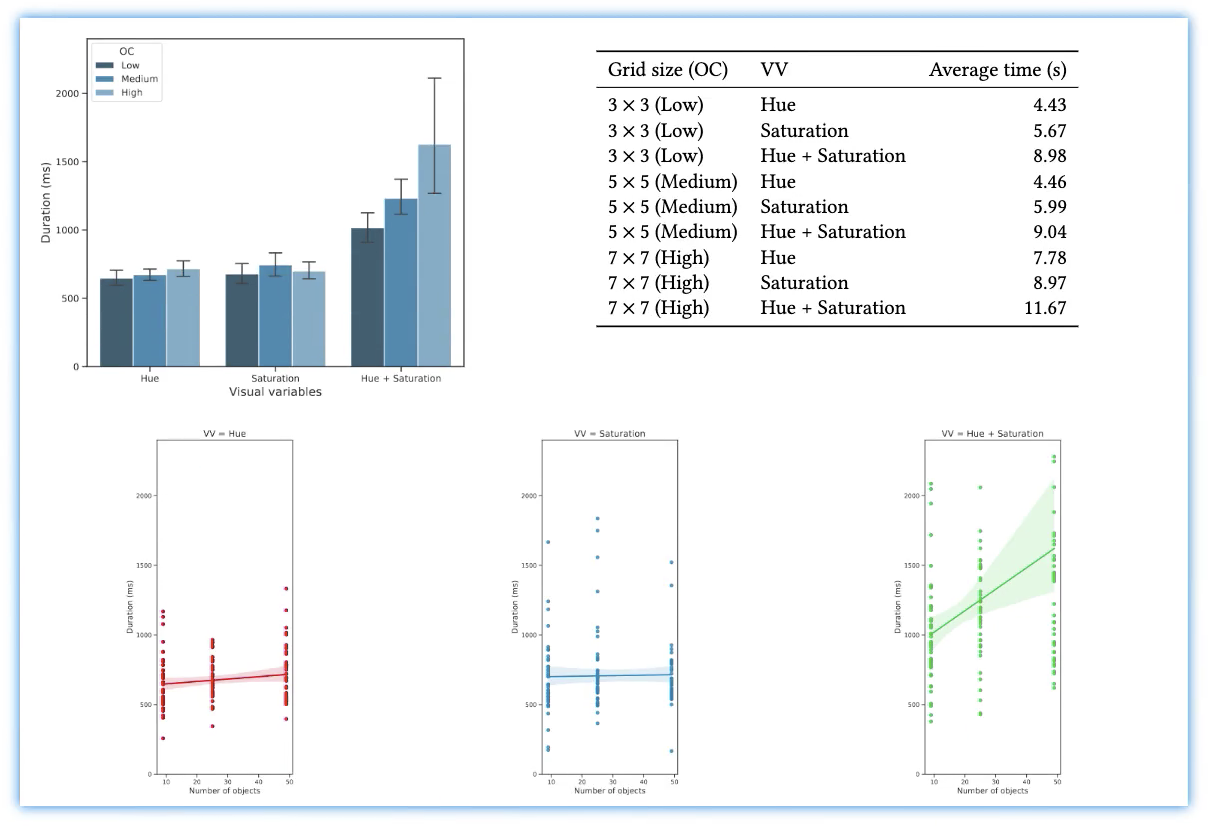
\includegraphics[height=\rowheight, width=\cellwidth, keepaspectratio]{grid-layout.png}
      \end{cell}
      \begin{cell}{0.5}
        \raggedright
        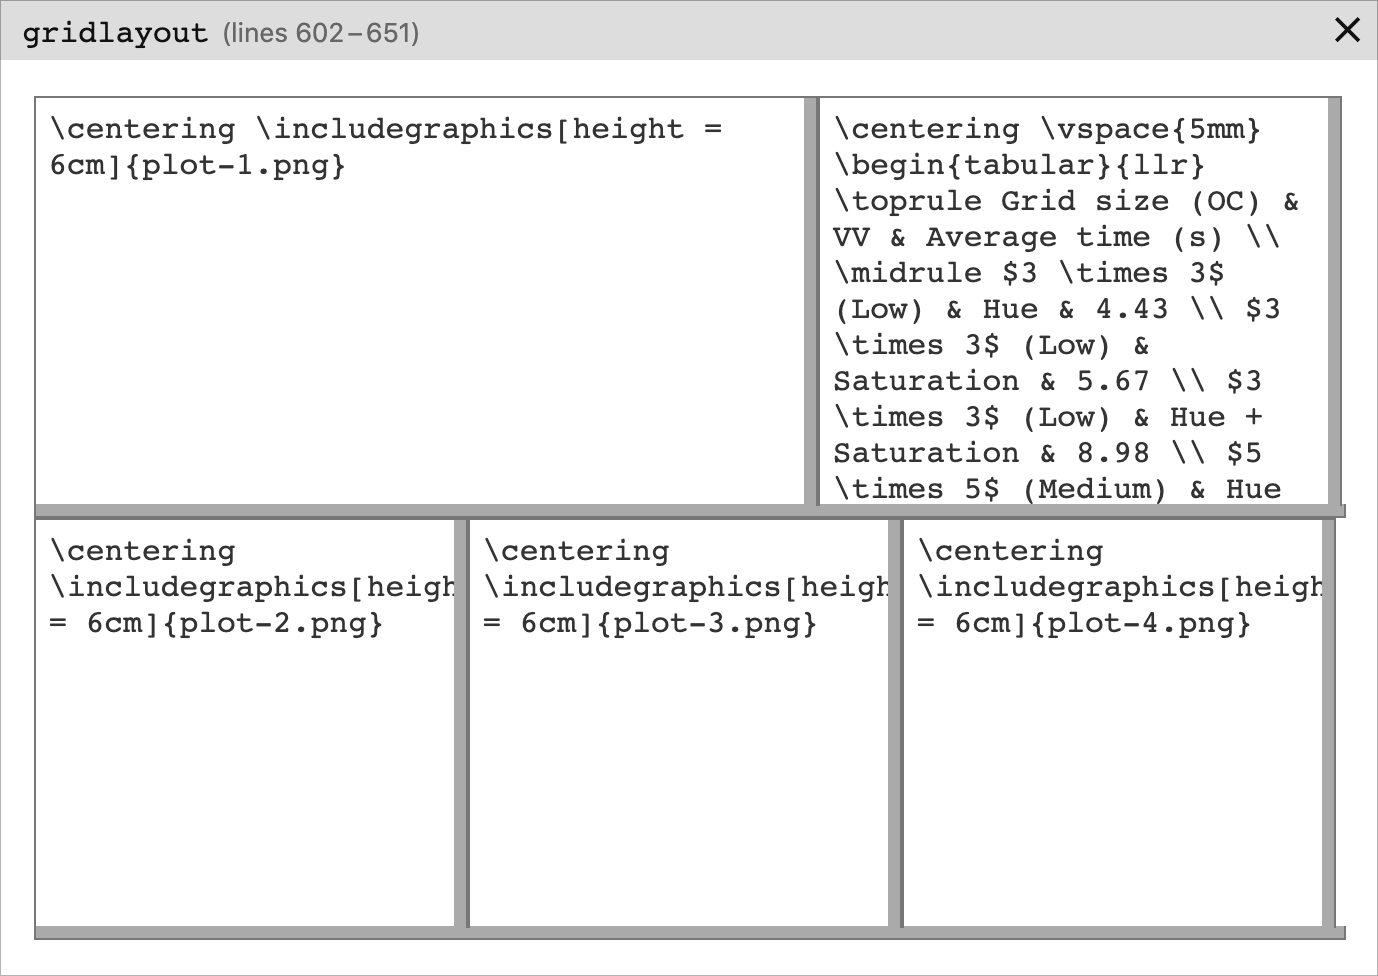
\includegraphics[height=\rowheight, width=\cellwidth, keepaspectratio]{grid-layout-vis.png}
      \end{cell}
    \end{row}
  \end{gridlayout}
  
  \caption{Exemples des visualisations disponibles dans \iLaTeX{}.
  Les éléments interactifs du PDF tels qu'ils apparaissent dans \iLaTeX{} sont affichés à gauche, et les visualisations du code les ayant générés sont affichées à droite (les images ne sont pas à l'échelle).
  Chaque visualisation ayant été modifiée, le code a déjà été mis à jour, et le document sera recompilé dès que la visualisation sera fermée. 
  \psubref{subfig:ilatex-visualisation-image} L'image a été rognée de façon à isoler le tableau central dans la visualisation --- d'où la région éclaircie en dehors du rectangle.
  \psubref{subfig:ilatex-visualisation-tableau} Les deux dernières colonnes ont été inversées dans la visualisation.
  \psubref{subfig:ilatex-visualisation-grille} La séparation entre les deux cellules de la première ligne a été déplacée vers la droite dans la visualisation.}
  \label{fig:ilatex-visualisations}
  \Description{Exemples d'une image, d'un tableau, d'une grille de mise en page et de leurs visualisations. La visualisation (a) contient une image dont une partie est sélectionnée dans un rectangle. La visualisation (b) contient le code des cellules du tableau sous forme de grille. La visualisation (c) contient le code de la grille sous forme d'une grille dont les dimensions sont proportionnées à celles de la grille issue du PDF.}
\end{figure*}



\subsection{Implémentation}
Le prototype est implémenté en tant qu'extension de l'éditeur Visual Studio Code\footnote{\url{https://code.visualstudio.com/}} (VSC), un éditeur de code open-source.
L'extension est écrite en TypeScript, HTML et CSS et organisée selon le patron de conception MVC.
Les particularités de son implémentation sont discutées ci-dessous.


\subsubsection{Extraction du code à visualiser}
Contrairement à la plupart des langages de programmation, \LaTeX{} n'est pas un langage hors-contexte, mais un langage récursivement énumérable (avec des caractéristiques peu communes telles que le concept de \emph{catcodes}, qui permet de modifier dynamiquement la signification de toute unité lexicale n'importe où dans le document).
En théorie, il est donc impossible d'écrire un analyseur syntaxique destiné à structurer le code que l'on souhaite visualiser en utilisant des outils traditionnellement dédiés à ce type de tâche.
Néanmoins, certaines conventions propres à \LaTeX{} demeurent très couramment utilisées (\eg{} la notion d'environnement).
En pratique, il est donc possible d'écrire un analyseur syntaxique qui accepte une proportion raisonnable de documents \LaTeX{} qui respectent lesdites conventions.

Pour les besoins du prototype, nous avons donc écrit un analyseur syntaxique de documents \LaTeX{} le plus générique possible dont le but est de fournir juste assez d'informations et de structure pour identifier les morceaux de code à visualiser, tels que certaines commandes spécifiques et leurs paramètres.
L'arbre de syntaxe abstraite ainsi généré est ensuite utilisé pour identifier les sous-arbres représentant des morceaux de code pertinents à visualiser (\eg{} un environnement nommé \texttt{tabular}).
Cette conception minimale a été choisie pour (1) maximiser le succès de l'analyse et (2) minimiser le temps d'exécution.
En contrepartie, chaque visualisation est responsable d'effectuer une analyse statique du code plus approfondie si nécessaire.


\subsubsection{Annotation du document PDF}
Le format de fichier PDF --- typiquement utilisé en sortie par les moteurs \LaTeX{} --- n'est pas conçu pour contenir des informations sur les régions du code \LaTeX{} à l'origine des différents éléments qui le composent.
Afin d'outrepasser cette limitation, nous avons choisi d'utiliser des annotations PDF contenant un identifiant unique et dont la boîte se superpose à celle de l'élément à associer à un morceau de code.
Celles-ci sont générées en englobant le morceau de code à visualiser dans une commande \texttt{ilatex} personnalisée\footnote{Bien que cela nécessite l'utilisation d'une commande spéciale pour le moment, il convient de noter que puisque tout peut être redéfini dans \LaTeX{}, les commandes et environnements existants pourraient être silencieusement modifiés afin que ceux-ci utilisent automatiquement la commande \texttt{ilatex}.}, comme dans \verb|\ilatex{\includegraphics{fig.pdf}}|.
Chaque utilisation de cette commande écrit également une nouvelle entrée dans un fichier regénéré à chaque compilation du document, qui contient des informations sur le morceau de code (\eg{} sa position dans le code) et sur la valeur courante de certaines macros (\eg{} \verb|\linewidth|).


\subsubsection{Affichage du PDF augmenté}
Une fois le document compilé en un PDF annoté, celui-ci est affiché à l'aide d'un moteur de rendu personnalisé (basé sur PDF.js\footnote{\url{https://github.com/mozilla/pdf.js/}}).
Celui-ci est responsable d'extraire toutes les annotations insérées par la commande \texttt{ilatex} et de les afficher sous forme de rectangles colorés autour des éléments disposant d'une visualisation.
Lorsque l'un d'eux est cliqué, \iLaTeX{} identifie le morceau de code auquel correspond l'annotation afin d'afficher la bonne visualisation.
Celui-ci est identifié en comparant l'identifiant attribué à l'annotation du PDF à ceux présents dans le fichier généré lors de la compilation du document.



\subsection{Évaluation préliminaire}
Étant donné la variabilité de l'expertise et des besoins de chaque utilisateur de \LaTeX{} (comme en attestent les différents profils des participants interviewés --- voir la {Table \ref{tab:participants}}), une étude quantitative de l'efficacité de \iLaTeX{} (\eg{} vitesse d'édition, nombre d'essais-et-erreurs) ne nous semble pas être très pertinente.
À l'inverse, une étude plus qualitative --- telle qu'une étude de terrain --- permettrait de mieux comprendre les contextes dans lesquels les RII sont préférées à l'édition du code et de découvrir des utilisations inattendues et des fonctionnalités manquantes.
Cependant, le contexte sanitaire en place depuis l'émergence de la pandémie de Covid-19 ne nous a pour l'instant pas permis d'organiser une telle évaluation.
En dépit de cela, une fois les interviews terminées, nous avons toutefois décidé de recueillir les avis des participants sur une vidéo d'une version précoce de \iLaTeX{} afin d'obtenir une première estimation de son potentiel.
Conscients du risque de biais dus à cette approche, nous avons fait particulièrement attention à ne pas parler du prototype ni de la notion de RII avant la fin de chaque interview.

\subsubsection{Méthodologie}
Nous avons présenté à chaque participant une vidéo d'un prototype de \iLaTeX{} d'une durée d'environ deux minutes.
Celle-ci présentait l'interface utilisateur du logiciel et l'utilisation de versions préliminaires des visualisations du code des images et des tableaux (semblables à celles présentées dans cette section).
La vidéo étant muette, nous expliquions chaque action en voix off à l'aide d'un script.
Une fois la vidéo terminée, nous avons demandé aux participants ce qu'ils avaient compris du système, s'ils aimeraient l'essayer, et s'il y avait d'autres types d'éléments du PDF ou de morceaux de code \LaTeX{} qu'ils souhaiteraient manipuler d'une façon similaire.
Ces évaluations ont été enregistrées dans les mêmes conditions que celles des interviews.

\subsubsection{Résultats}
La majorité des participants ont exprimé des réactions positives concernant la vidéo du prototype : \citeparticipant[P1]{Mais comment t'as codé ça ? C'est trop cool !} ; \citeparticipant[P7]{vend ton truc à Overleaf \elips{} qu'ils le rajoutent !}
Tous ont indiqué avoir compris le fonctionnement de \iLaTeX{}.
Plusieurs ont également fait la remarque que cela semblait facile à utiliser : \citeparticipant[P4]{c'est vachement intuitif, \elips{} ça fait référence à des compétences que les gens ont déjà} ; \citeparticipant[P8]{je pense que c'est plus user-friendly que juste modifier le code}.
Les utilisateurs les plus experts semblent eux aussi enthousiastes à l'idée d'utiliser le système.
P5 a d'ailleurs insisté sur le fait que \iLaTeX{} ne cherche pas à supprimer l'accès au code (\citeparticipant{si ce n'était pas comme ça je ne me verrais pas interagir avec}), et P11 a reconnu que \iLaTeX{} pourrait \citeparticipant[P11]{m'encourager à utiliser plus d'illustrations et de tableaux}.
En outre, P4 a souligné le potentiel pédagogique des visualisations : \citeparticipant{si je devais donner un cours sur \LaTeX{}, c'est un outil que j'utiliserais vraiment beaucoup je pense}, car il permet selon elle d'\citeparticipant[P4]{en apprendre un peu plus et un peu plus vite sur le code}.

Certains participants ont suggéré de nouvelles fonctionnalités pour les visualisations existantes (\eg{} sélectionner l'alignement horizontal des cellules d'une colonne de tableau), et plusieurs d'entre eux ont également mentionné qu'ils aimeraient avoir un contrôle plus direct sur les positions et les marges des différents éléments de leurs documents --- motivant ainsi le développement ultérieur de l'environnement \texttt{gridlayout}.
Quelques participants ont estimé qu'ils n'interagiraient que peu avec les visualisations de code peu compliqué (\eg{} les paramètres de la commande \texttt{includegraphics}), mais qu'ils seraient beaucoup plus intéressés par le système si celui-ci permettait de visualiser le code d'autres types de contenu.
Les exemples recueillis comprennent les figures composées de plusieurs sous-figures (P4), les molécules créées avec le paquet \texttt{chemfig} (P7), la configuration du style des éléments bibliographiques en éditant directement l'un d'entre eux (P6), et l'édition localisée des longues formules mathématiques (P9).
En outre, il est intéressant de noter que très peu de participants ont exprimé le souhait de pouvoir interagir avec le PDF dans le but de mettre en forme le document --- allant ainsi dans le sens de la distinction entre RII et WYSIWYG.



\subsection{Limitations}
Bien que le prototype fonctionne dans sa forme actuelle, celui-ci souffre de plusieurs limitations qui en font plutôt une preuve de concept.
D'une part, bien que la grammaire reconnue par l'analyseur syntaxique puisse être facilement étendue pour détecter l'utilisation d'autres commandes ou environnements (\eg{} pour faire une RII de listes implémentées avec les environnement \texttt{itemize} et \texttt{enumerate}), celle-ci ne permet pas de reconnaître certaines constructions (\eg{} les commandes utilisant des chevrons dans les présentations Beamer).
D'autre part, les trois visualisations que nous avons implémentées sont limitées en terme de fonctionnalités (\eg{} pas de fusion de cellules de tableau) et de robustesse (\eg{} tous les types de colonne ne sont pas supportés).

En outre, une évaluation plus systématique et longitudinale de \iLaTeX{} est nécessaire pour mieux comprendre les apports et les limites des RII pour l'édition de langages de description de document.
Néanmoins, bien que les avis que nous avons récoltés ne permettent pas de conclure de manière définitive sur l'apport en utilité ou en efficacité de \iLaTeX{}, il mettent en évidence l'intérêt que des utilisateurs de \LaTeX{} semblent porter aux RII --- soulignant l'importance de mener une évaluation plus approfondie d'un tel système.